\subsection{Konzept Grau}
Konzept Grau besteht aus drei Phasen:
\begin{itemize}
	\item \textbf{A - Vereinzelung mittels Schöpfrohrbunker:}
	Ein Schöpfrohrbunker dient zur Vereinzelung von Kugeln. Dabei werden NemaCaps in einem trichterförmigen Behälter (Punkt 2 in Abbildung \ref{fig:konzept_grau}) gesammelt. Zu unterst im Trichter befindet sich ein Rohr (1), welches eine Translation ausübt. Durch die Translation wird das unterste Gefüge so bewegt, dass ein oder mehrere NemaCaps ins Rohr fallen. So werden die NemaCaps in einer Reihe geordnet.
	
	\item \textbf{B - Auslösen und Transport mittels Pneumatik:}
	Aufeinander gestapelt, werden die NemaCaps von der Auslösung abgefertigt. Dabei wird das unterste NemaCaps mit einer linearen Bewegung (3) zu einer Öffnung geschoben. Zusätzlich wird das NemaCap an der Öffnung durch ein Vakum angesaugt. Durch einen Schlauch wird das NemaCap mittels Pneumatik zur Einsetzlokalität transportiert. 
	
	\item \textbf{C - Setzen mittels Rohr:}
	Zeitgleich zu Phase A und B wird am Topf das Setzen der NemaCaps vorbereitet. Dafür wird ein Rohr (4) in den stehenden Topf bis zur Setztiefe eingetaucht. Ist dieser eingetaucht, wird das NemaCap durch die Pneumatik zum Rohrende transportiert und somit im Topf platziert. Das Rohr fährt aus dem Topf, der Prozess beginnt von vorne.
\end{itemize}

Die Konfiguration des Setzmechanismus wird dabei durch die radiale Verstellung der einstechenden Rohre gewährleistet. Hierfür ist die manuelle Einstellung des Rohrs in radialer Richtung notwendig und vor jedem Batch auszuführen.

Dabei muss gewährleistet sein, dass das eintauchende Rohr nicht durch Erdpartikel verstopft wird.
\begin{figure}[H]
	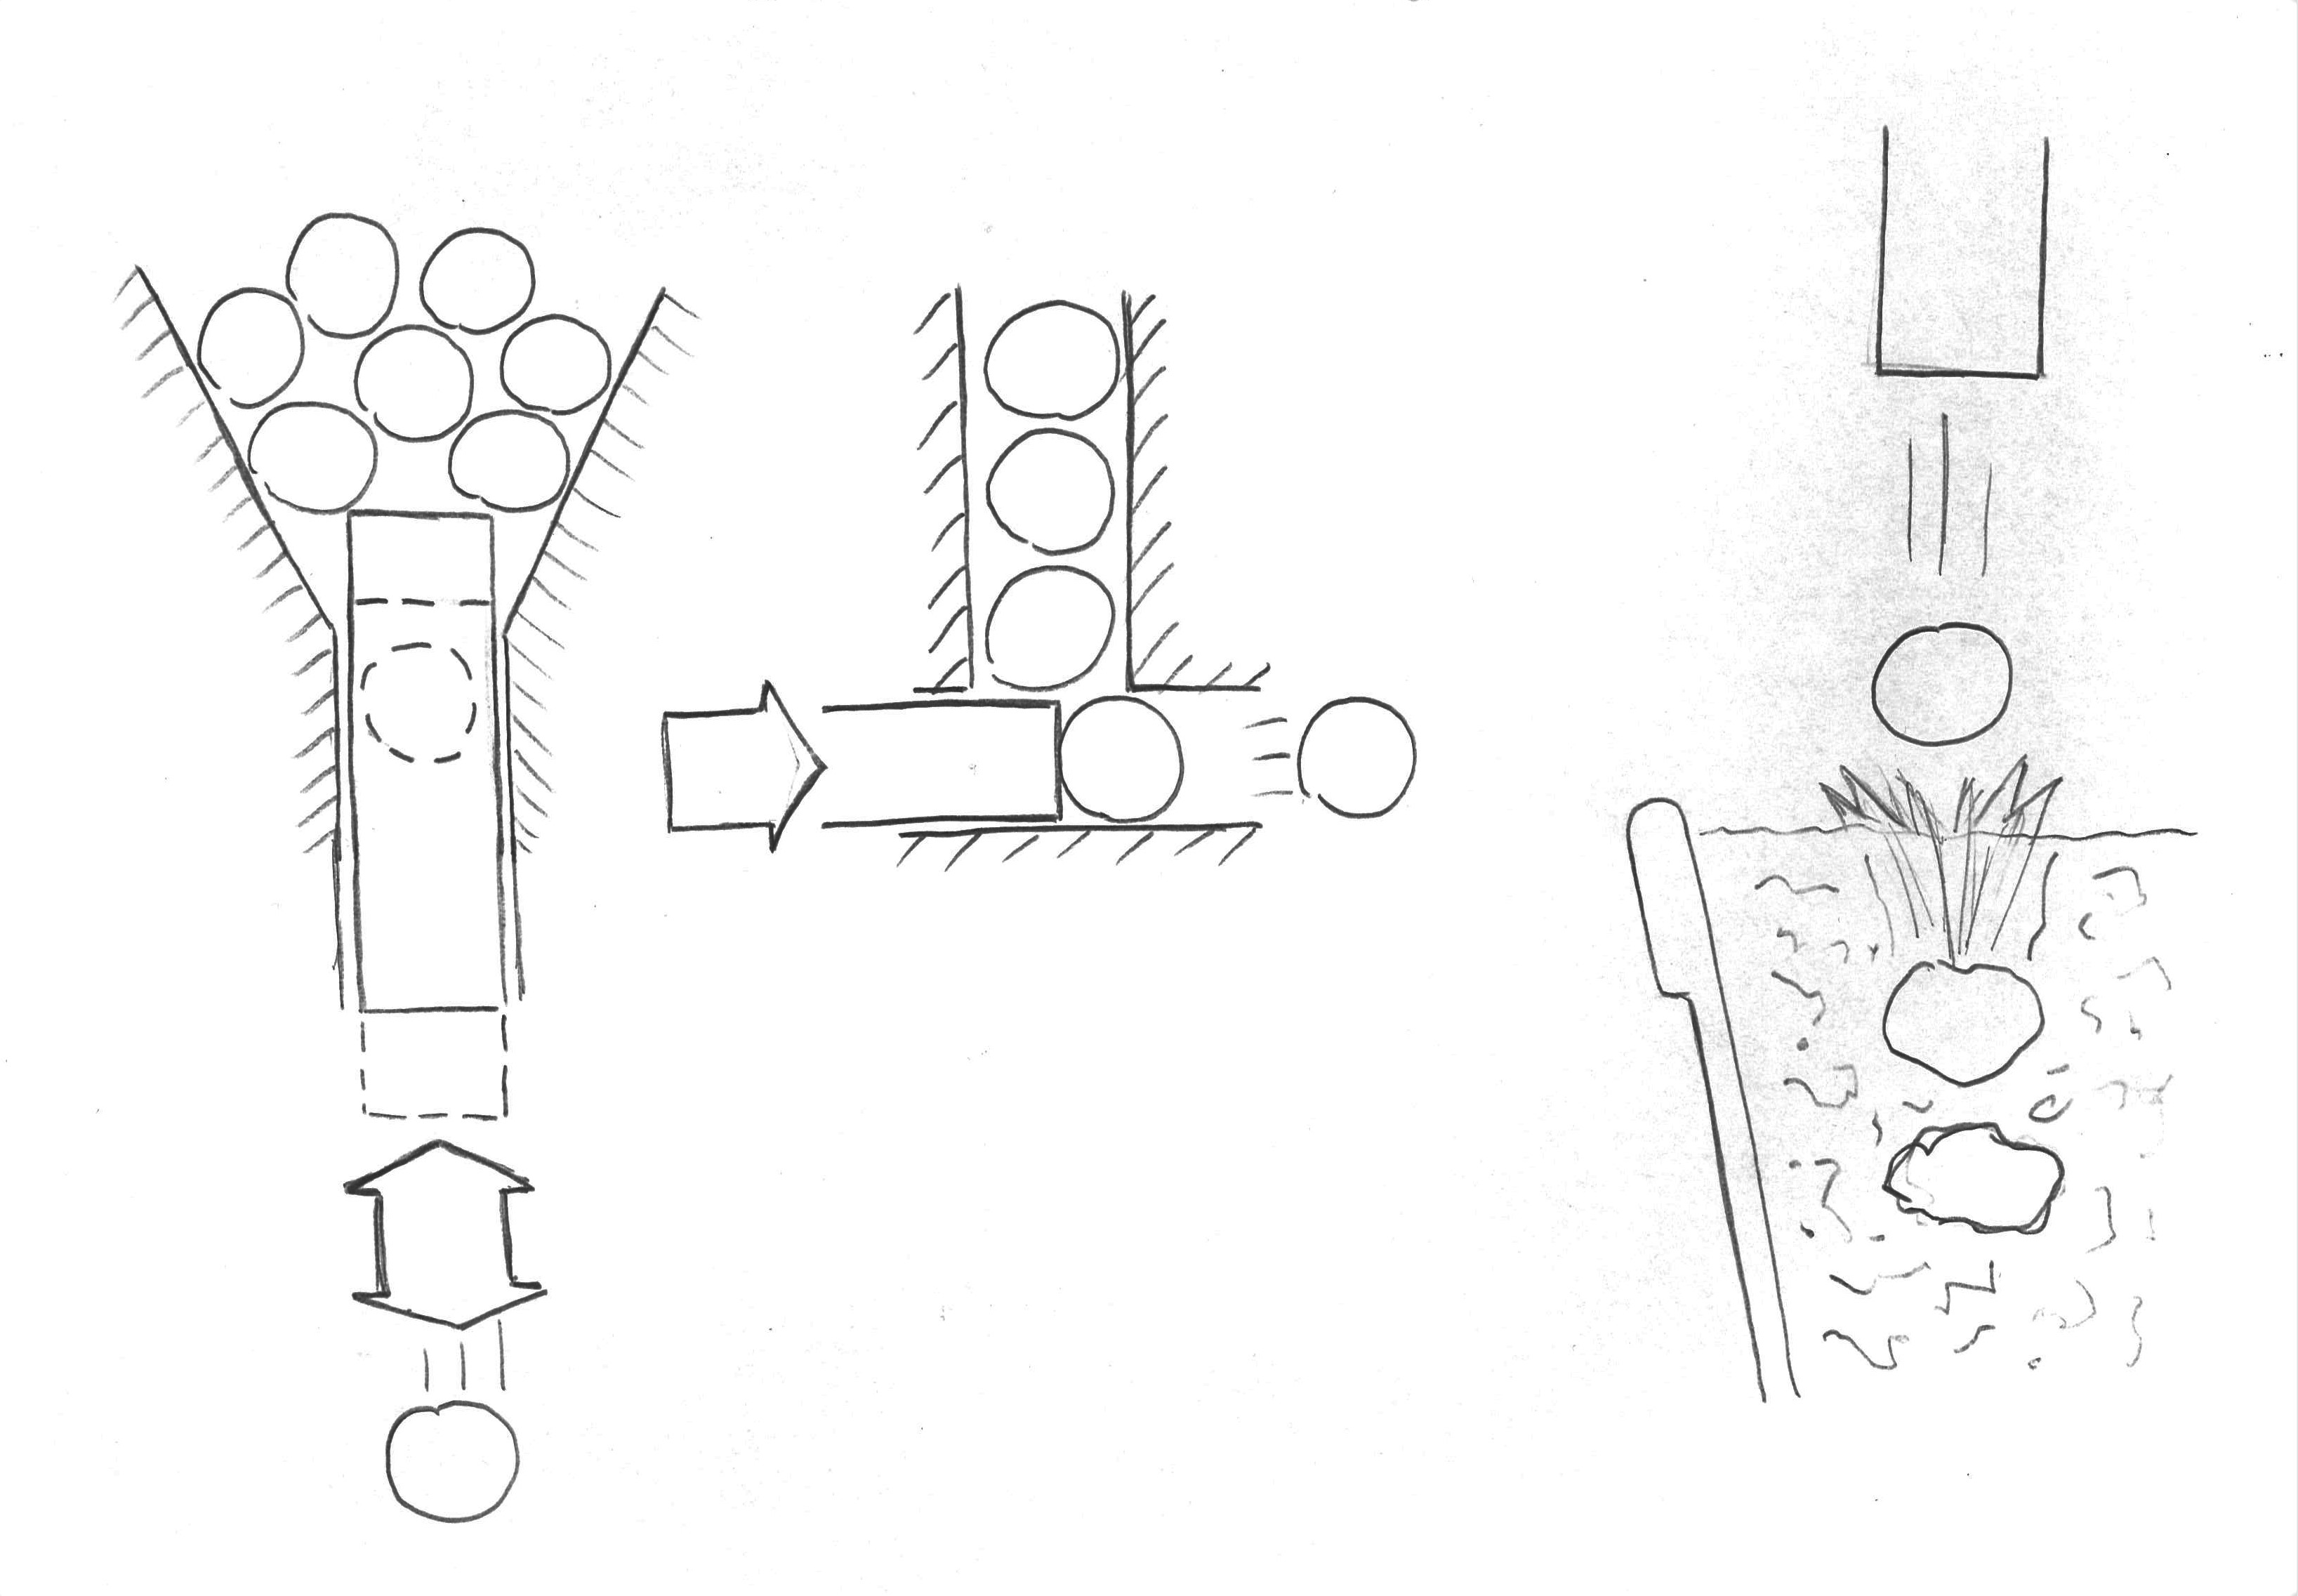
\includegraphics[scale=0.6]{Illustrationen/5-Konzept/grau_Konzept.jpg}
	\caption{Konzeptskizze von Konzept Grau}
	\label{fig:konzept_grau}
\end{figure}
